


\chapter{Neural networks} \label{ch:intro}
%Write somekind of introduction to the chapter before writing in the respective chapters
\begin{itemize}
    \item An introduction as to why neural networks are used as the tool for natural language processing
\end{itemize}

\section{Natural Language Processing using Neural Networks} \label{sec:NLProcNN}

\begin{itemize}
    \item In short, explain the advancement in the NLP department using neural networks
    \item Shortly introduce the concept of transformers
\end{itemize}

\section{Transformers} \label{sec:TF}

\begin{itemize}
    \item Explain the concept of transformers using a transformers diagram
    \item Explain shortly how the transformer model is trained
    \item Explain what makes it better than other model types (RNNs and CNNs)
\end{itemize}

\begin{figure}[h]
    \centering
    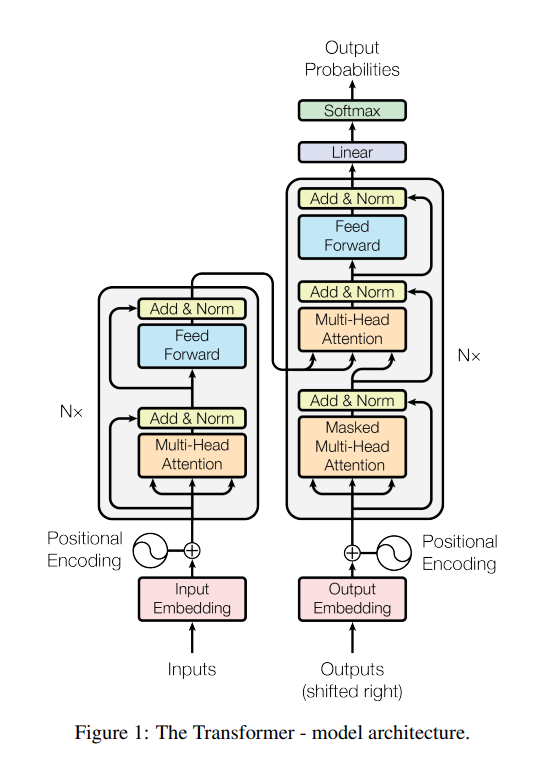
\includegraphics[width=8cm]{img/Transformers_TEMP.png}
    \caption{temporary transformers image}
   
\end{figure}


\section{Encoder models} \label{sec:ED}

\begin{itemize}
    \item Explain the concept of encoder models
    \item Explain how a transformer can be used as an encoder
    \item Go into how the encoder models has been advancing lately by introducing BERT and shortly explain what makes bert different than the normal transformer (Maybe bring in GLUE benchmarks)
    \item Tie up in the end by stating that Transformer based encoder models are the primary model type in the Stanza pipeline \textcolor{red}{Figured out that this is probably the case! :D}
\end{itemize}




